\chapter{Further Discuss on prediction method}
\label{ch:futuerDiscuss}


This chapter is about more test on the previous test conclusions. Here I just compare the top 3 method, that is Random Forest, Logistic Regression and SVM in stock direction prediction, Linear Regression, ANN and Random Forest in stock price accuracy test. All test are based on two years historical data

\section{Does Stock Price have effects on stock prediction results?}
\label{sec:priceInfluence}
To further discuss this topic, more test is needed. This section, stock tested number extend to 37 (newly added stock is list in table~\ref{tb:stock_list}), the testing result is showed in figure~\ref{fg:furtherCDC} and \ref{fg:furtherMAPE}. 


\begin{figure}[h]
	\centering
	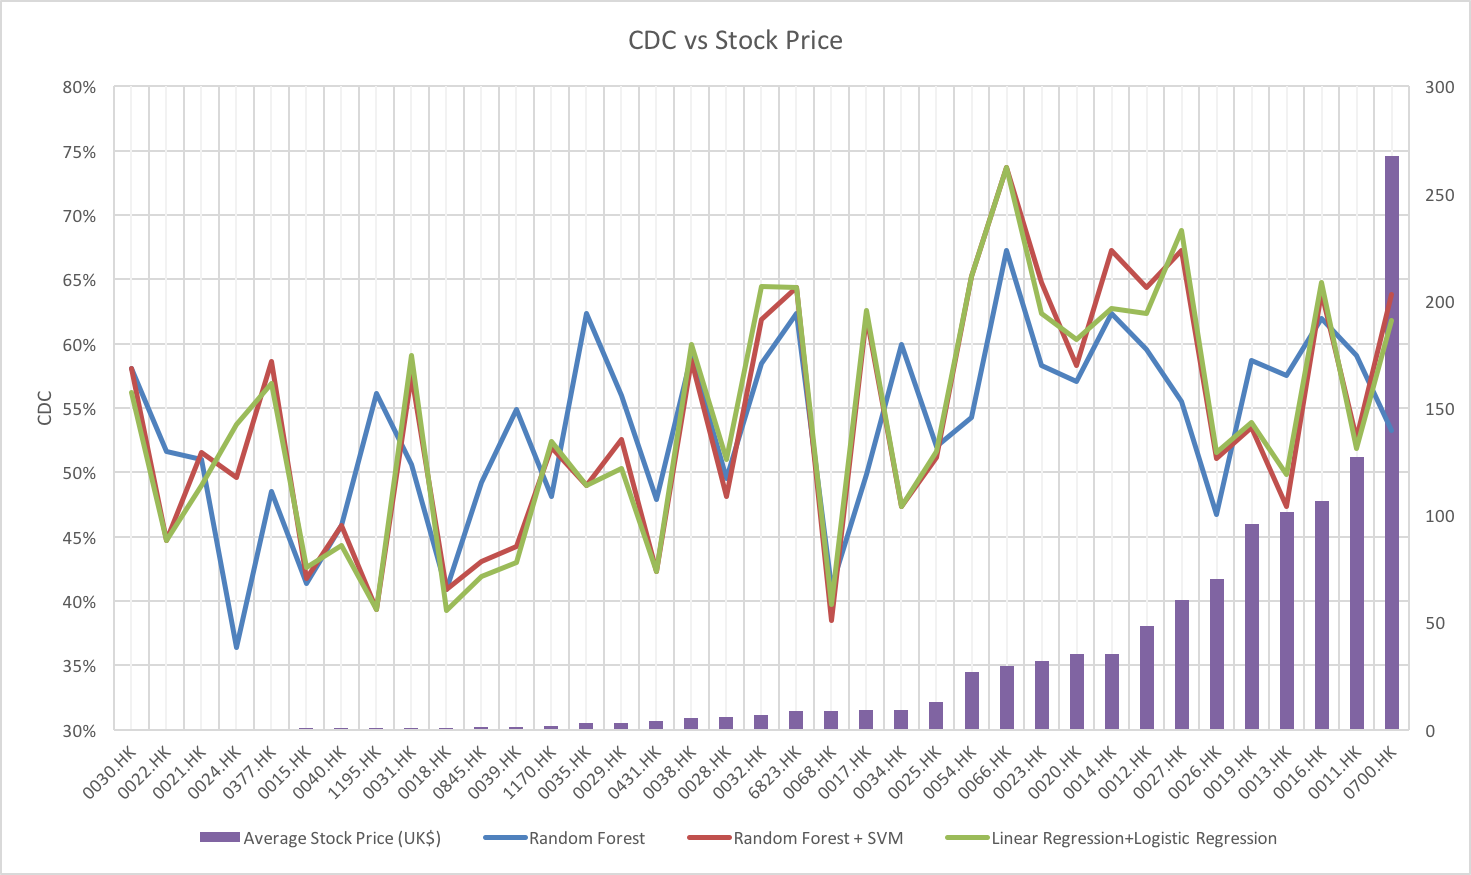
\includegraphics[width=0.8\textwidth]{FurtherDiscuss/CDCAVG}
	\caption{Extend result about stock price and CDC}
	\label{fg:furtherCDC}
\end{figure}


\begin{figure}[h]
	\centering
	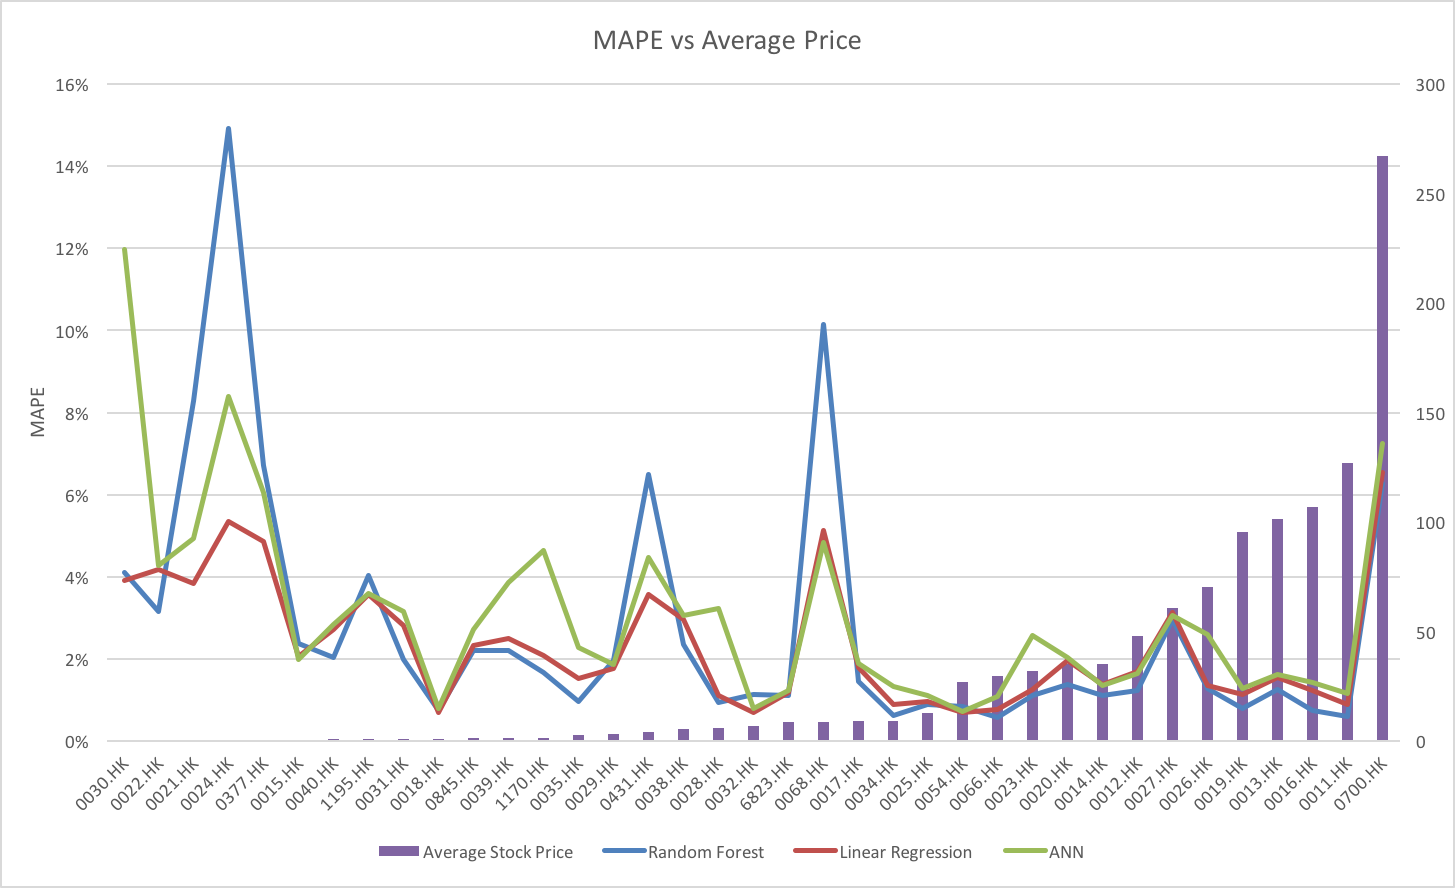
\includegraphics[width=0.8\textwidth]{FurtherDiscuss/MAPEAVG}
	\caption{Extend result about stock price and MAPE}
	\label{fg:furtherMAPE}
\end{figure}
\clearpage

The results show that stock price do not have relationship with the prediction result. It is true that MAPE of lower stock price seems to be larger than that of higher ones, this is because MAPE tends to have overestimate errors. For example, 0024.HK (Average stock price is \$0.37281405 during the testing period), the MAPE of using Random Forest to predict its price is 14.92\%, its MAD is just 0.054, still a very small value.\\


All methods tends to reach its best performance at the same stock. For example, the CDC of 0066.HK, 6823.HK, 0014.HK, 0016.HK, 0012.HK, 0038.HK, 0032.HK, 0023.HK, 0030.HK, 0027.HK is above 60\% while using all method. This stock also performs well in its MAPE test. On the other hand, 0018.HK, 0068.HK, 0015.HK have a poor performance. Does it happens to be so? Or it is because the chosen input data is more suitable to predict those stock?


\section{Stock Performance on Specific Stocks with different time period}
This section is tried to answer the question, stock tested in this section is the stock with good and bad performance in section~\ref{sec:priceInfluence} add 0002.HK, which also have a good performance in Chapter~\ref{ch:AccuracyResult}.\\


The data slot is from 2013-01-06 to 2016-01-06 (former two years as training data and later 1 years as testing data, training dataset size is 472, testing is 247).